%%% LaTeX Template
%%% This template can be used for both articles and reports.
%%%
%%% Copyright: http://www.howtotex.com/
%%% Date: February 2011

%%% Preamble
\documentclass[paper=a4, fontsize=11pt]{scrartcl}	% Article class of KOMA-script with 11pt font and a4 format


\usepackage[italian]{babel}															% English language/hyphenation
\usepackage[protrusion=true,expansion=true]{microtype}				% Better typography
\usepackage{amsmath,amsfonts,amsthm}										% Math packages
\usepackage[pdftex]{graphicx}														% Enable pdflatex
%\usepackage{color,transparent}													% If you use color and/or transparency
\usepackage[hang, small,labelfont=bf,up,textfont=it,up]{caption}	% Custom captions under/above floats
\usepackage{epstopdf}																	% Converts .eps to .pdf
\usepackage{subfig}																		% Subfigures
\usepackage{booktabs}																	% Nicer tables
\usepackage[latin1]{inputenc}
\usepackage{listings}
  \usepackage{courier}

%%% Advanced verbatim environment
\usepackage{verbatim}
\usepackage{fancyvrb}
\DefineShortVerb{\|}								% delimiter to display inline verbatim text


%%% Custom sectioning (sectsty package)
\usepackage{sectsty}								% Custom sectioning (see below)
\allsectionsfont{%									% Change font of al section commands
	\usefont{OT1}{bch}{b}{n}%					% bch-b-n: CharterBT-Bold font
%	\hspace{15pt}%									% Uncomment for indentation
	}

\sectionfont{%										% Change font of \section command
	\usefont{OT1}{bch}{b}{n}%					% bch-b-n: CharterBT-Bold font
	\sectionrule{0pt}{0pt}{-5pt}{0.8pt}%	% Horizontal rule below section
	}


%%% Custom headers/footers (fancyhdr package)
\usepackage{fancyhdr}
\pagestyle{fancyplain}
\fancyhead{}														% No page header
\fancyfoot[C]{\thepage}										% Pagenumbering at center of footer
\renewcommand{\headrulewidth}{0pt}				% Remove header underlines
\renewcommand{\footrulewidth}{0pt}				% Remove footer underlines
\setlength{\headheight}{13.6pt}

%%% Equation and float numbering
\numberwithin{equation}{section}															% Equationnumbering: section.eq#
\numberwithin{figure}{section}																% Figurenumbering: section.fig#
\numberwithin{table}{section}																% Tablenumbering: section.tab#



\usepackage{color}
\usepackage{xcolor}
\usepackage{listings}

 \lstset{
         basicstyle=\footnotesize\ttfamily, % Standardschrift
         %numbers=left,               % Ort der Zeilennummern
         numberstyle=\tiny,          % Stil der Zeilennummern
         %stepnumber=2,               % Abstand zwischen den Zeilennummern
         numbersep=5pt,              % Abstand der Nummern zum Text
         tabsize=2,                  % Groesse von Tabs
         extendedchars=true,         %
         breaklines=true,            % Zeilen werden Umgebrochen
         keywordstyle=\color{red},
    		frame=b,         
 %        keywordstyle=[1]\textbf,    % Stil der Keywords
 %        keywordstyle=[2]\textbf,    %
 %        keywordstyle=[3]\textbf,    %
 %        keywordstyle=[4]\textbf,   \sqrt{\sqrt{}} %
         stringstyle=\color{white}\ttfamily, % Farbe der String
         showspaces=false,           % Leerzeichen anzeigen ?
         showtabs=false,             % Tabs anzeigen ?
         xleftmargin=17pt,
         framexleftmargin=17pt,
         framexrightmargin=5pt,
         framexbottommargin=4pt,
         %backgroundcolor=\color{lightgray},
         showstringspaces=false      % Leerzeichen in Strings anzeigen ?        
 }
\lstloadlanguages{% Check Dokumentation for further languages ...
         %[Visual]Basic
         %Pascal
         %C
         %C++
         %XML
         %HTML
         %Java
{[Sharp]C}
 }
\usepackage{caption}
\DeclareCaptionFont{white}{\color{white}}
\DeclareCaptionFormat{listing}{\colorbox{gray}{\parbox{\textwidth}{#1#2#3}}}
\captionsetup[lstlisting]{format=listing,labelfont=white,textfont=white}

%%% Title	
\title{ \vspace{-1in} 	\usefont{OT1}{bch}{b}{n}
		\huge \strut Implementazione del gioco del Bantumi \strut \\
		\Large \bfseries \strut Corso di Intelligenza Artificiale 2012 \strut
}
\author{ 									\usefont{OT1}{bch}{m}{n}
        Nicola Febbrari\\		\usefont{OT1}{bch}{m}{n}
        Universit\`a degli Studi di Verona\\	\usefont{OT1}{bch}{m}{n}
        Facolt\`a MM.FF.NN.\\
        \texttt{nicola.febbrari@studenti.univr.it}
}
\date{22 gennaio 2013}

%%% Begin document
\begin{document}
\maketitle
\section{Introduzione}
Con questo progetto vorrei mettere in pratica alcune  tecniche che sono state spiegate durante il corso di intelligenza artificiale, pertanto, ho deciso di realizzare il gioco del Bantumi implementando un algoritmo di intelligenza artificiale per poi confrontarlo con altri programmi analoghi.

\section{Il Gioco}
Il Bantumi \`e un antico gioco da tavolo di origine africana, composto da una tavola in legno con 12 buche disposte su due file parallele e due buche pi\`u grandi, una per giocatore, dette granai.
Si gioca in due, in partenza ogni giocatore possiede 18 semi che dispone uniformemente nelle proprie buche (3 in ogni buca), lasciando i 2 granai vuoti.
A turno, ogni giocatore pu\`o effettuare una mossa che consiste nello scegliere una propria buca non vuota, prendere tutti i semi che contiene e distribuirli, in senso antiorario, uno in ogni buca successiva, utilizzando anche il granaio e le buche dell'avversario (granaio avversario escluso).



\begin{figure}[h]
\centering
        \includegraphics[totalheight=4.4cm]{Bantumi.png}
    \caption{Tavola.}
    \label{fig:verticalcell}
\end{figure}

\section{Altre regole}
\begin{enumerate}
	\item Un giocatore non pu\`o mai depositare semi nel granaio dell'avversario
	\item Se l'ultimo seme, tra quelli da distribuire, viene depositato nel proprio granaio, il giocatore ha diritto ad un ulteriore turno.

\begin{figure}[h]
\centering
        \includegraphics[totalheight=3cm]{Bantumi_4.png}
    \caption{Turni multipli.}
    \label{fig:verticalcell}
\end{figure}
	\item Se l'ultimo seme viene depositato in una propria buca senza semi, il giocatore prender\`a questo seme e tutti i semi della buca di fronte dell'avversario e li metter\`a nel proprio granaio.

\begin{figure}[h]
\centering
        \includegraphics[totalheight=3cm]{Bantumi_2.png}
    \caption{Raccolta.}
    \label{fig:verticalcell}
\end{figure}
\begin{figure}[h]
\centering
        \includegraphics[totalheight=3cm]{Bantumi2.png}
    \caption{Cattura.}
    \label{fig:verticalcell}
\end{figure}

	\item Il gioco termina quando tutte le buche di un giocatore sono vuote. Terminato il gioco il giocatore con pi\`u semi nel granaio \`e il vincitore.
\end{enumerate}

\section{Implementazione del Gioco}
\subsection{I progetti.}
Ho strutturato il codice dividendolo in 4 progetti:
\begin{itemize}
	\item \textit{Bantumi.entities.interface}: il progetto in cui sono contenute tutte le interfacce delle entit\`a;
	\item \textit{Bantumi.entities}: l'implementazione di tutte le classi;
	\item \textit{Test}: il progetto di unit test per il test automatico durante il processo di TDD;
	\item \textit{UI Console}: il progetto per la user interface.
\end{itemize}

\subsection{Le entit\`a}
Le principali entit\`a per la realizzazione del gioco sono:
\begin{itemize}
	\item La classe \textit{Tavola}, che descrive la tavola fisica, le buche e i semi contenuti;
	\item Le classi \textit{Player}, che descrivono le varie implementazioni dei giocatori;
	\item La classe \textit{Gioco}, che implementa le regole e i vincoli del Bantumi;
	\item La classe \textit{Bantumi}, che si occupa del set-up.
\end{itemize}


\section{Implementazione dell'algoritmo di IA}
\subsection{Implementazione MinMaxPlayer}
Per implementare un giocatore con intelligenza artificiale ho utilizzato uno degli algoritmi per la \textit{ ricerca con avversari} visti a lezione, l'algoritmo \textit{ MinMax}.
\paragraph{Definizioni}
\begin{itemize}
\item L'\textit{albero} rappresenta la combinazione di tutte le possibili mosse eseguibili, partendo da una situazione consolidata della tavola di partenza.
\item Un \textit{nodo} dell'albero rappresenta una possibile mossa fatta dal giocatore di turno.
\item Il \textit{livello} dell'albero rappresenta tutte le possibili mosse (o sequenze di mosse nel caso di turno multiplo) che pu\`o eseguire il giocatore di turno.
\end{itemize}

\paragraph{Algoritmo}
Ad ogni turno l'algoritmo decide quale sia la mossa migliore. Partendo da una situazione consolidata della Tavola, vengono elaborati i valori di ogni mossa possibile usando un calcolo ricorsivo sugli stati successivi generati da tutte le possibili combinazioni di mosse valide.\\
La ricorsione percorre l'albero fino alle foglie, valuta il valore della foglia assegnandogli un +1 se la foglia rappresenta uno stato di vittoria, 0 se di pareggio o -1 in caso di sconfitta. 
Dopo aver calcolato il valore di una foglia viene fatto \textit{ backtracking} sull'albero di gioco eventualmente aggiornando la scelta del nodo ottimo \textit{ MinMax} in base al livello dell'albero (nel caso di turno proprio turno Max nel caso di turno dell'avversario Min).

\paragraph{Complessit\`a}
Per eseguire la ricerca viene fatta una vista in profondit\`a dell'albero di gioco. Nel Bantumi la dimensione dell'albero risulta ingestibile, infatti, se per ogni turno ci possono essere \textit{ m} mosse e una partita dura \textit{ t} turni, nello stato iniziale scorrere tutto l'albero ha una complessit\`a in tempo di $O(m^t)$.

\subsection{Alfa Beta pruning}
La dimensione dell'albero di gioco del Bantumi nelle prime mosse \`e troppo grande e rende impossibile l'esplorazione, questo \`e dovuto proprio all'esponenzialit\`a rispetto al numero di turni. Ovviamente non \`e possibile ridurre il problema ad una complessit\`a trattabile (polinomiale), tuttavia utilizzando un meccanismo di potatura possiamo evitare di valutare porzioni di albero che sicuramente non verranno prese in considerazione durante la fase di decisione della mossa migliore.\\ 
L'idea \`e quella di valutare ad ogni nodo, dato un determinato stato possibile della tavola, se c'\`e uno stato predecessore che risulta essere migliore. Se questo fosse verificato ovviamente renderebbe inutile la valutazione di questa porzione di albero
\begin{lstlisting}[label=maxPruning,caption=Implementazione Max con taglio]
//Array delle mosse ordinete secondo una funzione Euristica
int[] heuristc = _heuristicFunction.HeuristicFunction(gioco.Clone());
for (int j = 0; j < heuristc.Length; ++j)
{
    int i = heuristc[j];
    OperationCount++;
	//Clono il gioco
    IGioco giocoClone = gioco.Clone();
	//Eseguo la mossa
    giocoClone.Muovi(i);
	//Verifico se la mossa ha causato un cambio turno
    bool cambioTurno = gioco.ProssimoTurno != giocoClone.ProssimoTurno;
    ValoreMossa valoreProssimaMossa = null;
	//Condizione di uscita dalla ricorsione
    if (!giocoClone.Finito)
    {
		//Se non cambia il turno continuo con il Max
        if (!cambioTurno)
		{
			//Chiamata ricorsiva passo la profondità (per limitare l'albero) e alfa(migliore scelta per MAX)/beta(migliore scelta per MIN)
            valoreProssimaMossa = MaxValue(giocoClone, depth, alfa, beta);
		}
        else
		{
            valoreProssimaMossa = MinValue(giocoClone, depth + 1, alfa, beta);
		}
    }
	//Calcolo il valore della mossa	
    ValoreMossa valore = new ValoreMossa(valoreProssimaMossa, i, ValoreAttuale(giocoClone));
    if (null == resultMove)
    {
        resultMove = valore;
    }
    else
    {
        resultMove = AggiornoValore(resultMove, valore, latoStep);
    }
	//Non verra' mai scelto da MIN  e fermo il ciclo
    if (resultMove.Valore > beta && cambioTurno)
        return resultMove;
	//Se e' un valore migliore per MAX aggiorno alfa
    alfa = resultMove.Valore > alfa ? resultMove.Valore : alfa;
}\end{lstlisting}

Un ruolo fondamentale per la qualit\`a dei tagli eseguiti durante l'algoritmo \`e dato dalla funzione euristica. Scegliendo una buona funzione \`e possibile dare dei valori significativi ad alfa beta durante i primi cammini, cos\`i da riuscire a tagliare grosse porzioni di albero e risparmiare cicli di computazione.
Nel caso del Bantumi ho implementato questa funzione basandomi sul risultato della differenza fra il valore dei due granai calcolato per ogni mossa possibile. Le mosse con una differenza maggiore vengono valutate prima.
\subsection{Limitazione della profondit\`a}
La potatura alfa beta non \`e stata sufficiente per ridurre l'elaborazione a tempi accettabili, quindi ho deciso di introdurre nell'algoritmo un parametro che limitasse la dimensione dell'albero. Ho deciso di parametrizzare quanti passii espandere l'albero (un passo comprende i 2 turni dei giocatori).
\subsection{Studio dell'apertura}
Un'ultimo perfezionamento che ho fatto \`e stato quello di studiare le mosse di apertura. Ho fatto giocare contro s\`e stesso il mio Bot, impostando livelli di esplorazione elevati che hanno richiesto molte ore di computazione. Una volta analizzate le prime due mosse sono riuscito ad aumentare notevolmente la capacit\`a di vittoria anche utilizzando Bot con livelli di esplorazione bassi.
\subsection{Conteggio operazioni}
Completate tutte le implementazioni ho cercato di fare delle valutazioni empiriche cercando di confrontare gli algoritmi e le varie euristiche che ho implementato per capire se effettivamente i miglioramenti teorici che avevo ipotizzato hanno avuto degli effetti.
Per la valutazione ho eseguito un conteggio del numero dei nodi esaminati partendo da una situazione neutra rappresentata dalla tavola iniziale. Come prima cosa ho eseguito il test sull'algoritmo MinMax, variando la limitazione del numero di turni.
\begin{table} [h]
    \begin{tabular}{lccc}
        \hline
        Algoritmo & Senza Hueristic & Heuristc Desc\footnotemark[1] & Heuristc Val\footnotemark[2]\\ \hline
        MinMax(1) & 129 & ~ & ~ \\ 
        MinMax(2) & 8727 & ~ & ~ \\ 
        MinMax(3) & 882215 & ~ & ~ \\ 
        MinMax(4) & 99569593 & ~ & ~ \\ 
        MinMaxAlfaBeta(1) & 112 & 83 & 97 \\ 
        MinMaxAlfaBeta(2) & 3057 & 2209 & 2405 \\ 
        MinMaxAlfaBeta(3) & 84577 & 56770 & 50387 \\ 
        MinMaxAlfaBeta(4) & 2676841 & 1320574 & 1148562 \\ 
        MinMaxAlfaBeta(5) & 81995855 & 25298451 & 23123673\\ 
        \hline


    \end{tabular}
\end{table}
\footnotetext[2]{I nodi vengono scelti per la valutazione in modo decrescente}
\footnotetext[3]{I nodi vengono scelti con una funzione euristica che valuta il valore in base alla differenza fra i due granai pi\'u  0,5 se la scelta d\`a diritto ad una seconda mossa}
\begin{figure}[h]
\centering
        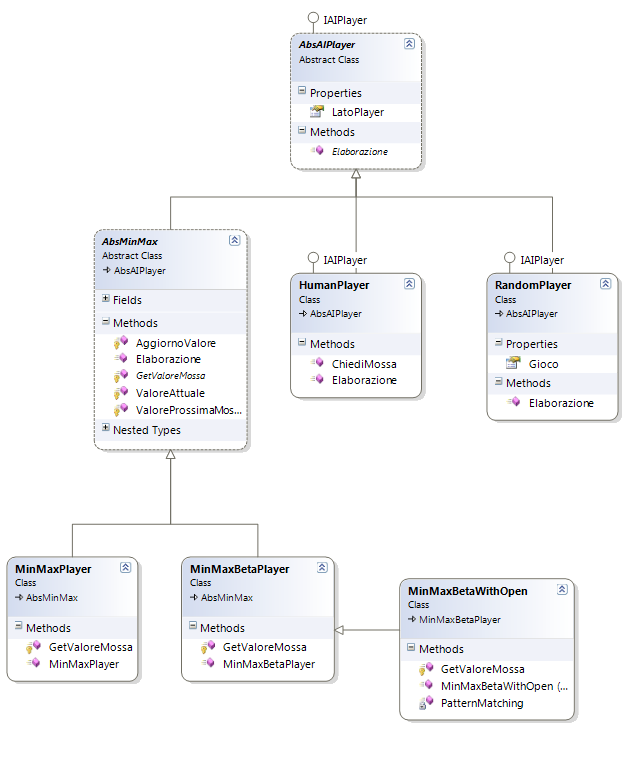
\includegraphics[totalheight=18cm]{Iplayer.png}
    \caption{Diagramma delle classi dei Players implementati.}
    \label{fig:verticalcell}
\end{figure}

\subsection{Osservazioni}
Confrontando i risultati ottenuti con le implementazioni realizzate si pu\`o immediatamente osservare il grande vantaggio computazionale dato dall'introduzione dell'alfabeta pruning. Con 4 passi di gioco (8 turni) senza nessuna potatura i nodi valutati sono quasi 100M, mentre a parit\`a di profondita, ma utilizzando una funzione euristica di ordinamento nella scelta della potatura, i nodi analizzati sono poco piu di 1M. Questo risultato cos\`i evidente mi fa ipotizzare che con uno studio approfondito delle tecniche di gioco sia possibile implementare una funzione euristica migliore che ottimizzi i tagli per poter estendere ulteriormente la profondit\`a dell'albero.
\section{Bot a confronto}
Per una valutazione finale dell'implementazione ho confrontato l'algoritmo con alcuni giochi del Bantumi presenti in commercio. Questi sono i risultati:
\begin{table} [h]
    \begin{tabular}{llc}
        \hline
        Player1 & Player2 & Vincitore \\ \hline
	
	MinMaxAlphaBetaWithOpen(1) & kalahandroid 1.2	&	kalahandroid\\
	MinMaxAlphaBetaWithOpen(2) & kalahandroid 1.2	&	kalahandroid\\
	MinMaxAlphaBetaWithOpen(3) & kalahandroid 1.2	&	MinMax\\
	kalahandroid 1.2    & MinMaxAlphaBetaWithOpen(3)& 	PARI \\
	kalahandroid 1.2    & MinMaxAlphaBetaWithOpen(4)& 	MinMax \\
	MinMaxAlphaBetaWithOpen(3) & Mancala-Gold 	&		MinMax\\
	MinMaxAlphaBetaWithOpen(3) & Bantumi Atomic Pineapple& MinMax\\
	MinMaxAlphaBetaWithOpen(3) & Bantumi FREE Paul Production &MinMax\\
	MinMaxAlphaBetaWithOpen(3) & Nicola 			&MinMax\\
	Nicola & MinMaxAlphaBetaWithOpen(3) 		&	MinMax \\
	Nicola & MinMaxAlphaBetaWithOpen(1) 		&	MinMax \\

        \hline

    \end{tabular}
\end{table}
\section{Risultati e sviluppi futuri}
Il progetto \`e stato strutturato cercando di mantenere una forte indipendenza fra l'infrastruttura del gioco e l'implementazione dei vari algoritmi di IA. Questa scelta mi ha permesso di sperimentare diverse strategie, di procedere con un miglioramento graduale degli algoritmi scritti, ma soprattutto di poter consolidare in modo semplice e immediato alcuni concetti teorici spiegati durante il corso.\\
Il normale completamento del progetto sarebbe la realizzazione di una interfaccia utente web/mobile che utilizza il mio progetto per realizzare la IA; una possibile evoluzione del core, invece, potrebbe essere quella di sperimentare qualche tecnica di calcolo distribuito per sfruttare la potenza computazionale che potrebbe mettere a disposizione un' infrastruttura di cloud computing.
\end{document}